\documentclass{novanarrative}


\newenvironment{storyquote}
{
\noindent\begin{minipage}[t]{1.0\linewidth}\centering
\begin{tikzpicture}
\node (t) at (0,0) \bgroup
\begin{minipage}[c]{5.5in}\centering\Large\usefont{T1}{ostrichblack}{m}{n}
}
{\end{minipage}
\egroup;
\node[above = -1.5em of t] {
\includegraphics{art/rules/rule-top.pdf}};
\node[below = -1.5em of t] {
\includegraphics[angle=180]{art/rules/rule-top.pdf}};
\end{tikzpicture}
\end{minipage}
}

\newenvironment{storyquotepage}
{
\clearpage
\squelchbackground
\thispagestyle{empty}

\vbox to 0pt{}
\vfill
\begin{storyquote}
}
{
\end{storyquote}
\vfill
\vbox to 0pt{}

\pagebreak

\restorebackground
}



\begin{document}
\squelchbackground
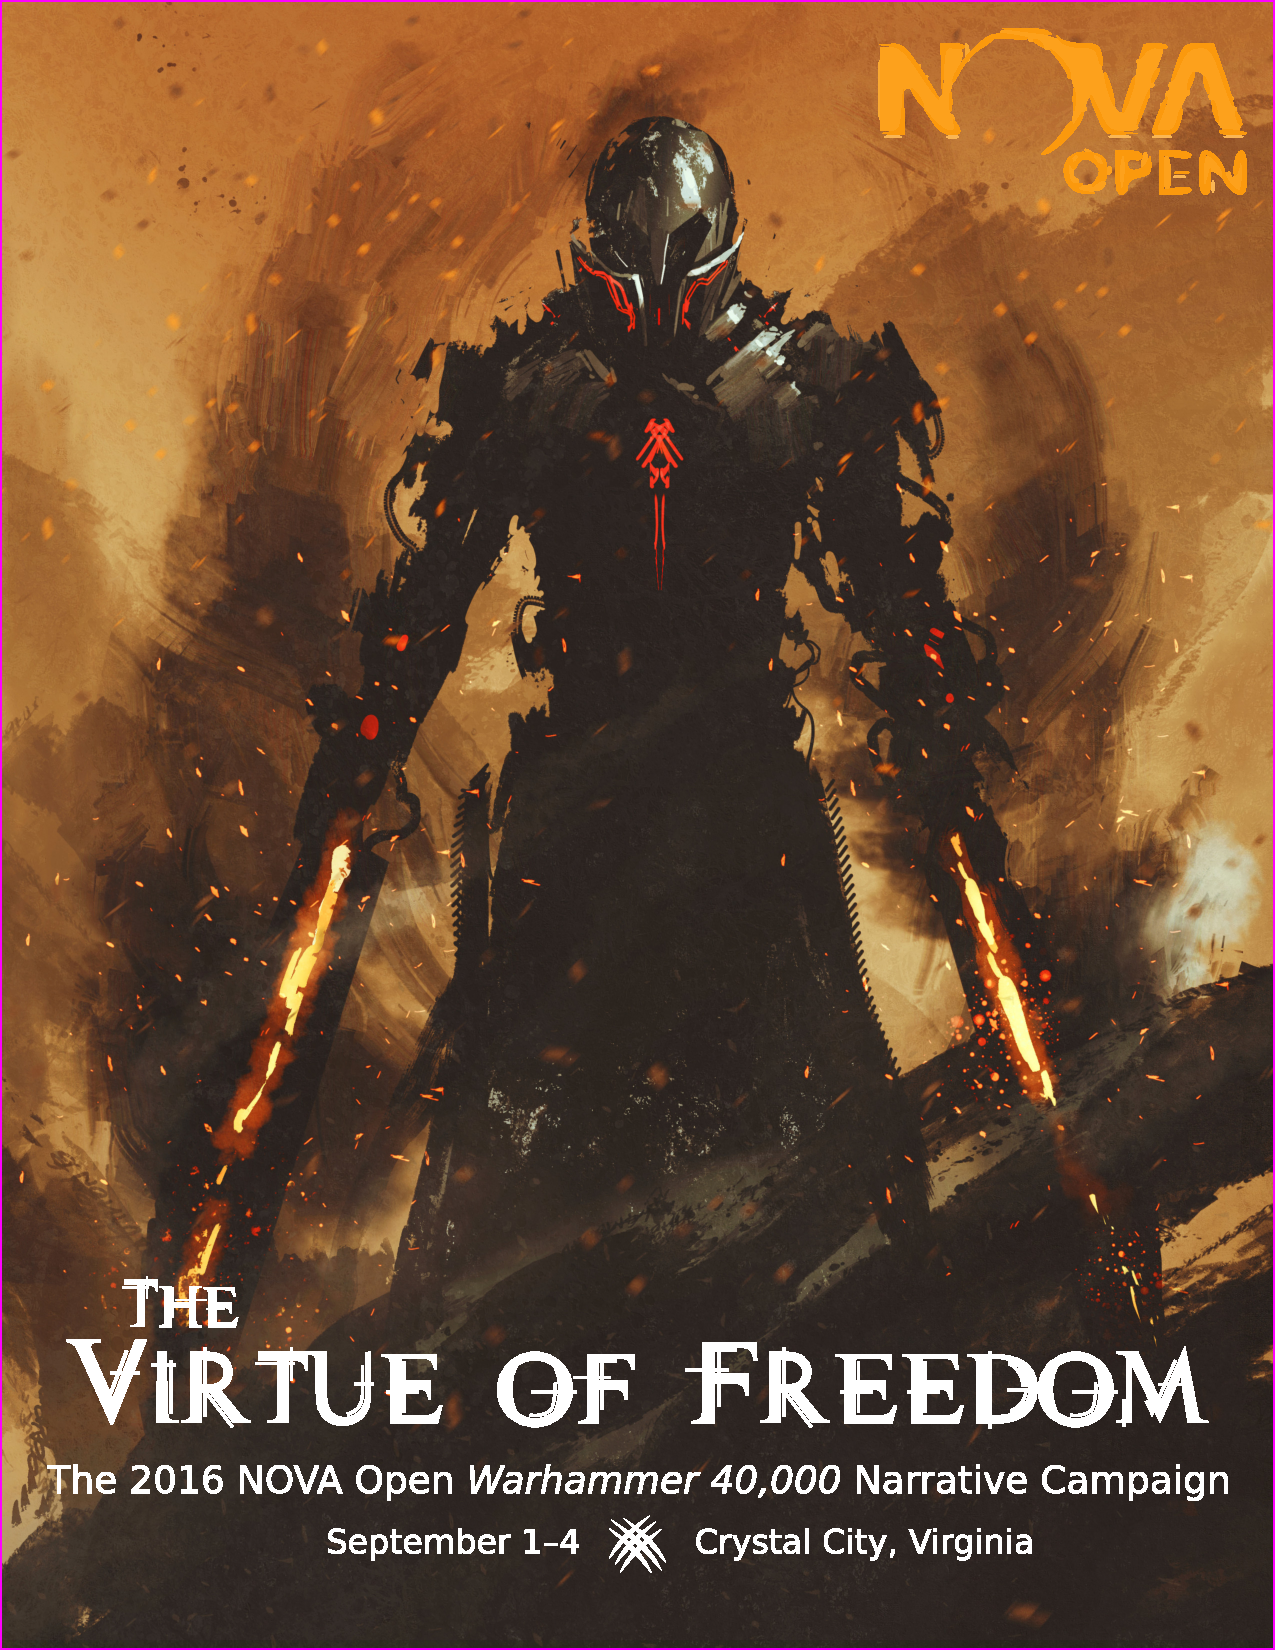
\includepdf[pages={1},fitpaper,offset=0cm 0cm]{art/cover/cover}
\pagebreak
\restorebackground

%%----------------------------------------------------------------------
%%----------------------------------------------------------------------
\begin{storyquotepage}  
  The Virtue society was founded amid chaos and bloodshed, war and
  betrayal.  Species fought species, worlds fought worlds, beings
  fought beings.  Violence was unceasing, ruthless.  The virtues and
  our adherence to them saved us.  Discipline, order, peace, these
  gave us a path forward.

  \bigskip And yet, along that path, we forgot one:\\
  The virtue of freedom.

  \bigskip - Sanctioned poet-in-exile Shossola,\\Commentaries
\end{storyquotepage}

%\setcounter{page}{1}
\chapter{Introduction}

Welcome to another year of the NOVA \textit{Warhammer 40,000}
Narrative!

The NOVA 40k Narrative is a high quality wargaming experience based on
an ongoing story in an original science fiction universe.  It is
team-centric, with players organizing into two alliances and
collectively making strategic decisions such as match pairings and
targets.  Most importantly, it is a narrative campaign, not a
tournament.  Stellar play and notable achievements are recognized, but
the focus is on social gaming with a strong narrative tilt.  Missions
aren't necessarily symmetric, and some of them aren't even fair.
Opponents also may or may not be working toward covert objectives of
which you're not even aware, or have a secret resource or stratagem
that they or their alliance won in earlier battles.  If your driving
motivation is competition and winning games, this event is not for
you.  If your main interest though is having fun, playing good games
with great people, and making your mark on a multi-year story built by
hundreds of fellow 40k gamers, then this is where you want to be
September 1--4, 2016.

Going into its fifth year, our player-created storyline continues with
The Virtue suffering the after-effects of its failed assault on Earth,
defeated by Humanity over the course of the previous events.  Whether
you're a new rookie or a returning veteran: Strap in, check your ammo,
and brace for impact---eons old, galaxy spanning civilizations don't
change easily.  Join us now for the 2016 NOVA 40k Narrative:

\bigskip
\centerline{
\includegraphics{art/title/title.pdf}}

\section{Updates}

This year's 40k Narrative is going to continue the things you love
about it.  But a number of changes and improvements are also being
made.  Primary gameplay updates of which to be aware include the
following:

\begin{itemize}
%\item The opposing sides in the story have broadened.

\item Registration will be simplified and balancing of the sides
  improved, with players signing up for the event as a whole and then
  joining a side on opening night.

\item Codex-specific Narrative Supplements have been dropped.  They're
  too unwieldy to balance and maintain under Games Workshop's current
  hectic release schedule, as likely to imbalance armies as balance
  them, and skewed registration toward one or the other side in order
  to get specific boosts.

\item Players will instead customize their armies through selecting a
  Technical Skill, such as Field Medicine, Electronics, or
  Assassination.  These will provide small, thematic in-game boosts;
  notable advantages toward specific narrative mission objectives; and
  a player-specific campaign progression.

\item Not everyone will be playing the same mission in each round,
  instead choosing from several options to meet the strategic needs of
  their side and to best match their technical skill and army list.

\item Superheavy vehicles and gargantuan creatures with at most~9
  HP/Wounds are permitted.

\item An optional Quick Reaction Force detachment is made available to
  use in army lists.
\end{itemize}

\section{Release Schedule}

There are a number of significant components to the NOVA 40k
Narrative.  This player guide will be extended over the coming months
as they are developed, tested, and released.  The following milestones
are the latest by which you can expect details on those components.

\begin{center}  
\begin{tabular}{C{1.5in}L{5in}}
\rowcolor{LineColor}\textbf{\color{white} Date} & \multicolumn{1}{c}{\textbf{\color{white} Changes}}\\
  January 1 & Event schedule and basic army selection rules\\
  March 1 & Background story, campaign mechanics, and sample mission\\
  May 1 & Technical skills list, personal scoring, and painting contest rules\\
  July 1 & Public mission book, resources and stratagems samples\\
  September 1 & \textit{Game on!}\\
\end{tabular}
\end{center}


\section{Changelog}

This table summarizes what has been changed in each release of this document.

\begin{center}  
\begin{tabular}{C{1.5in}L{5in}}
  \rowcolor{LineColor}\textbf{\color{white} Date} & \multicolumn{1}{c}{\textbf{\color{white} Changes}}\\
  January 31, 2016 & Schedule tweaked to better accommodate seminars.  Quick Reaction Force detachment made more restrictive.  Basic gameplay rules were added (invisibility, rerollable 2+ saves, team games).\\
  \rowcolor{LightGray} January 1, 2016 & Initial public release.
\end{tabular}
\end{center}


%%----------------------------------------------------------------------
%%----------------------------------------------------------------------
\chapter{Event Schedule}

There are two registration and participation tracks in the NOVA 40k Narrative:
\begin{itemize}
\item \textbf{Warlords.} Six amazing, storyful games, from Thursday
  night to Sunday mid-day, and war council meetings to make strategic
  decisions such as match objectives and pairings.

\item \textbf{Nightfighters.} Three great games on Thursday, Friday,
  and Saturday night.  This is a good option for players who want to
  participate in the 40k Narrative, but also play in NOVA 40k GT or
  other events.
\end{itemize}

The following table provides the detailed schedule for both tracks.

\begin{center}  
\begin{tabular}{C{0.75in}C{0.75in}C{2in}L{3in}}
\rowcolor{LineColor}\textbf{\color{white} Day} & \textbf{\color{white} Time} & \textbf{\color{white} Participants} & \multicolumn{1}{c}{\textbf{\color{white} Activity}}\\
  Thursday & 20:30 & Warlords \& Nightfighters & Joint Briefing \& Match Pairings\\
           & 21:30 & Warlords \& Nightfighters & \textbf{Battle Round 1}\\
\\
\rowcolor{LightGray} Friday     & 10:00 & Warlords                  & Alliance War Councils\\
\rowcolor{LightGray}            & 10:30 & Warlords                  & Match Pairings\\
\rowcolor{LightGray}            & 11:00 & Warlords                  & \textbf{Battle Round 2}\hfill\textit{(to 13:30)}\\
\rowcolor{LightGray}            & & & \\
\rowcolor{LightGray}            & 16:30 & Warlords                  & Joint Briefing\\
\rowcolor{LightGray}            & 17:00 & Warlords                  & Alliance War Councils\hfill\textit{(to 18:00)}\\
\rowcolor{LightGray}            & & & \\
\rowcolor{LightGray}            & 20:30 & Warlords \& Nightfighters & Joint Briefing \& Match Pairings\\
\rowcolor{LightGray}            & 21:30 & Warlords \& Nightfighters & \textbf{Battle Round 3}\\
\\
                     Saturday   & 10:00 & Warlords                  & Alliance War Councils\\
                                & 10:30 & Warlords                  & Match Pairings\\
                                & 11:00 & Warlords                  & \textbf{Battle Round 4}\hfill\textit{(to 13:30)}\\
                                & & & \\
                                & 16:30 & Warlords                  & Joint Briefing\\
                                & 17:00 & Warlords                  & Alliance War Councils\hfill\textit{(to 18:00)}\\
                                & & & \\
                                & 20:30 & Warlords \& Nightfighters & Joint Briefing \& Match Pairings\\
                                & 21:30 & Warlords \& Nightfighters & \textbf{Battle Round 5}\\
\\
\rowcolor{LightGray}   Sunday   & 10:30 & Warlords                  & Joint Briefing\\
\rowcolor{LightGray}            & 11:00 & Warlords                  & Alliance War Councils\\
\rowcolor{LightGray}            & 11:30 & Warlords                  & Match Pairings\hfill\textit{(to noon)}\\
\rowcolor{LightGray} & & & \\
\rowcolor{LightGray}            & 13:00 & Warlords                  & \textbf{Battle Round 6}\hfill\textit{(to 15:30)}\\
\rowcolor{LightGray}            & 16:30 & Warlords \& Nightfighters & Joint Briefing: Outcomes!\hfill\textit{(to 17:00)}\\
\end{tabular}
\end{center}


%%----------------------------------------------------------------------
%%----------------------------------------------------------------------
%\begin{storyquotepage}  
%  Even the smallest of daggers can cause the\\gravest of wounds if they
%  come from behind.
%
%\bigskip
%- Attribution lost,\\Chronicles of Foundation,\\restricted historical draft
%\end{storyquotepage}

\makeatletter\@openrightfalse
\chapter{Army Selection}
\@openrighttrue\makeatother

Each player must prepare two army lists:

\begin{itemize}
\item \textbf{Campaign Force.} For your individual battles, the
  majority of the campaign.\hfill\textit{Up to 2000 points.}

\item \textbf{Strike Force.} For your team games, of which there will
  be at least one.\hfill\textit{Up to 1000 points.}
\end{itemize}

Both army lists must be battle forged.  No model with more than~9 hull
points or wounds is permitted.  Superheavy vehicles and gargantuan
creatures are otherwise allowed.

The strike force list need not be a subset of the campaign force list,
but cannot include any factions not utilized in the campaign force
list.  As detailed below, in team games you will have your own
warlord, and your units will count as allies of convenience to those
of your partner(s), regardless of factions.

No other requirements or constraints are placed on detachments,
formations, or force organization. An optional Quick Reaction Force
detachment is made available for this event, described below.

\section{Sources}

Forgeworld units and armies eligible for standard \textit{Warhammer
  40,000}, i.e., not \textit{Apocalypse}, are permitted. Units and
armies from Forgeworld's Horus Heresy \textit{Age of Darkness} books
are also permitted.

All up-to-date, official \textit{Warhammer 40,000} army sources are
permitted that are available in current publication. This does include
White Dwarf entries, which are available via back issues, and current
campaign books. It does not include limited edition dataslates and
formations, e.g., those included in mega-bundles. Contact the
tournament organizer(s) beforehand about any questions. Remember that
you must have all sources on hand, electronically or digitally.

For any codex or supplement re-released within two weeks preceding the
event, you may choose whether to use the old or new edition. You may
not use both editions of a single source within the event.

\section{Models}

Models must be WYSIWYG, but identifiable and thoughtful conversions
and proxies are welcome. Indistinguishable or confusing proxies are
not acceptable.  Contact the organizer(s) beforehand for any
questions.

In addition, models need not be painted, but is \textit{very strongly}
recommended in order to not impair the experiences of all other
participants.  A painting component will be applied to personal scores
to reward finished armies, following the standardized NOVA metrics.



\section{Quick Reaction Force}

Players may optionally employ a Quick Reaction Force detachment in
their army lists, defined as follows.

\subsection{Force Organization}

An army may only contain a single Quick Reaction Force detachment.
All units in the detachment must have the same faction, or no faction.
The detachment is comprised of the following battlefield roles.

\begin{center}
\begin{tabular}{C{0.75in}C{0.75in}C{0.75in}C{0.75in}C{0.75in}C{0.75in}}
\rowcolor{LineColor}\textbf{\color{white} HQ}	& \textbf{\color{white} Troops}	& \textbf{\color{white} Elites}	& \textbf{\color{white} Fast Attack}	& \textbf{\color{white} Heavy Support}	& \textbf{\color{white} Lords of War}\\
1--2	& 2--6	& 1--4	& $\star$	& $\star$	& 0--1\\
\end{tabular}
\end{center}

A Quick Reaction Force detachment must include one Fast Attack and one
Heavy Support choice. It may include up to three selections in one of
those roles, but must contain one and only one selection in the other
role. I.e., the detachment must adhere to one of the following
options:

\begin{itemize}
\item 1--3 Fast Attack and 1 Heavy Support
\item 1 Fast Attack and 1--3 Heavy Support
\end{itemize}

As usual, dedicated transports are not counted toward these quantity limitations.

\subsection{Command Benefits}

The following advantages are granted for utilizing this detachment:

\begin{itemize}
\item \textbf{Objective Secured.} All scoring units in this detachment
  except superheavy vehicles and gargantuan creatures gain Objective
  Secured. A unit with this special rule controls objectives even if
  an enemy scoring unit is within range of the objective marker,
  unless the enemy unit also has this special rule.

\item \textbf{QRF Commander.} If this detachment is your primary
  detachment, instead of rolling a random warlord trait you may choose
  a warlord trait from the tables in the main \emph{Warhammer 40,000}
  rulebook.  If you wish to use a different table of warlord traits,
  i.e., from a codex, then you must roll a random trait, but may
  reroll the result.

\end{itemize}

%%----------------------------------------------------------------------
%%----------------------------------------------------------------------
\makeatletter\@openrightfalse
\chapter{Gameplay Rules}
\@openrighttrue\makeatother

This section defines the basic gameplay rules applied in the 40k Narrative.

\section{Core Rules}

The following rules apply to all games in the NOVA 40k Narrative.

Matches are scheduled for~2.5 hours, but players may take more time as
long as they mutually agree to do so.  Please discuss and come to a
decision on playing long or not at the start of each match, or at
least well before the time limit, so that there are no assumptions or
mismatched expectations.  This flexibility ensures that players may
participate in seminars and other NOVA events without hindering their
Narrative experience, but have the option to play at a relaxed pace if
they have no schedule constraints.  Results must be submitted at least
half an hour before the next activity on the Narrative schedule.

The Invisibility psychic power is amended to be:

\begin{center}  
\begin{tabular}{L{6in}}
\arrayrulecolor{LineColor}\hline\\
  \emph{Invisibility} is a blessing that targets a single friendly unit
  within 24". While the power is in effect, enemy units shooting at the
  target unit do so at BS 1, and in close combat will only hit models of
  the target unit on To Hit rolls of 5+.\\
\\
\arrayrulecolor{LineColor}\hline\\
\end{tabular}
\end{center}

For any failed 2+ save that may be rerolled, the reroll only succeeds on a 4+.

\section{Team Rules}

The rules in this section apply to team games in the 40k Narrative.

All players in a team field their strike force lists as separate
armies. \textbf{Regardless of factions, teammates consider their
  partners' units and models to be allies of convenience to their own
  army.}  In addition, all players on a team nominate a warlord for
themselves as usual.
%, thus a doubles pair would have two warlords in play.

Results rolled by a player on the Warp Storm table (\emph{Codex: Chaos
  Daemons}) do not affect their teammates' armies and models unless
specifically dictated by the table, i.e., other Chaos Daemons or
marked Chaos Space Marines.

In the psychic phase, a single D6 is rolled by the current team to
determine the base warp charge from which each player on both teams
generates their own individual pools, applying the usual rules to
their own models. Players all use their own warp charge pool;
teammates cannot combine or share warp charge. Any opposing player
with models on the table may attempt to deny the witch, caveat that if
a specific unit of enemy models is targeted, their player alone may
attempt to block the spell.

Units may not shoot at close combats even if none of their player's
units are engaged.

Teams are not eliminated unless there are no models of any member on
the table.

For all other gameplay purposes the combined forces of a team are
considered a single army comprised of multiple detachments, and the
team considered a single player for all rules except when specifically
distinguished by the missions here. How units belonging to different
players in a team interact are thus governed by the rules for allies
of convenience, on page 126 of the main \emph{Warhammer 40,000}
rulebook.


%%----------------------------------------------------------------------
%%----------------------------------------------------------------------
\begin{storyquotepage}  
  Who could have guessed this age, its unprecedented discord and
  dissent, would start with one small, unremarkable blue planet,
  itself already all but forgotten?

\bigskip
- Premiere Thyx,\\Transcripts of Governance Enclave TTTLAV.O
\end{storyquotepage}


%%----------------------------------------------------------------------
%%----------------------------------------------------------------------
\makeatletter\@openrightfalse
\chapter{Story So Far}
\@openrighttrue\makeatother

We pick up our tale in the future...

\bigskip
\begin{center}  
\begin{tabular}{L{6in}}
  \arrayrulecolor{LineColor}\hline\\
  {\it
  The Virtue is the greatest civilization ever arisen in the galaxy.
  More than a species, more than an empire, more than a philosophy; The
  Virtue is a way of being.  Its culture and technology
  are unsurpassed.  Its will is absolute.  The Virtue is perfect.

  \bigskip
  The Virtue \emph{was} perfect.

  \bigskip
  It has been two hundred years since The Virtue fought Humanity.  Their
  pacification forces were smashed, but at great cost to the human
  defenders.  Earth is a barren husk.  Its mighty war fleets have
  vanished, scattered to the solar winds if not lost entirely.  A paltry
  few survivors' colonies have integrated into the ignored, disordered, minor
  societies along the fringe worlds and outlaw regions at the edge of The Virtue's control,
  enduring as best they can
  in the shadow of the colossus.

  \smallskip
  The Virtue, for its part, has retreated into itself.  Effects of that
  failed conquest echo still, slowly rippling across the staid society.
  For the first time in millennia, murmurs of disquiet have been heard
  in the governance enclaves.  Questions flitter across the noosphere.
  How could a perfect society be defeated by such an unenlightened race?
  In a universe where everything is known, what could be unknown?

  \smallskip
  Spawned from this moral crisis, disparate elements on the perimeter of
  The Virtue's space have begun fomenting open rebellion.  Branding themselves
  the Coalition of the Free, their messages have appeared across
  message boards and even hastily graffitied in public spaces on the
  outer worlds, praising a new virtue:

  \bigskip
  \centerline{The virtue of freedom.}
  }
  \\
  \arrayrulecolor{LineColor}\hline\\
\end{tabular}
\end{center}

\section{The Past}

The~2016~40k Narrative continues the ongoing NOVA story of The Virtue
and Humanity.

\paragraph{NOVA 2012: First Contact.}  After a brush with global
nuclear war in~2194, humanity stepped back from the brink.  The
millennia-old dreams of scholars, tyrants, and preachers became a
reality as all the people of Earth finally set aside their
differences.  That peace was shattered a mere eighteen years later
when thousands of alien craft struck the planet without warning.
Millions died before any response could even begin.  Eventually though
a resistance formed.  Taking its last stand in Washington, D.C., the
defenders were dumbfounded when the invaders inexplicably retreated.

%\clearpage
\noindent\begin{minipage}[c]{(0.6\linewidth)-1em}%\vbox to 0pt{}
\paragraph{NOVA 2013: Cataclysm.}  Learning what they could from alien
captives and technology left behind, humanity strove to rebuild and
prepare.  Their caution was well founded: In~2312, one hundred years
to the day of the first invasion, the invaders struck again.  Against
much improved resistance and plagued by doubts, they once more though
faltered even as millions died.  Faced with defeat, their commander
rammed his flagship into Earth in a final ignominious gesture,
igniting its antimatter cores in the planetary mantle.  The blast and
shockwaves killed billions, with billions more lost in catastrophic
aftereffects.  Humanity survived merely through those few population
centers shielded enough to outlast the trauma.

\bigskip
\paragraph{NOVA 2014: Descension.} Regrouping in the aftermath,
humanity began a two-pronged offensive.  Space fleets began pushing
outward from Earth, learning much about the invaders and from where
they had come.  Forces on Earth meanwhile attempted to cleanse the
planet of the numerous aliens still fighting on.  This fight however
was doomed.  The planet had simply sustained too much damage, and the
numerous invaders still extant on the surface were only working to
further its destruction.  Eventually the cold truth became clear and
inevitable: The Earth was truly lost.
\end{minipage}\hfill%
\begin{minipage}[c]{0.4\linewidth}%\vbox to 0pt{}
  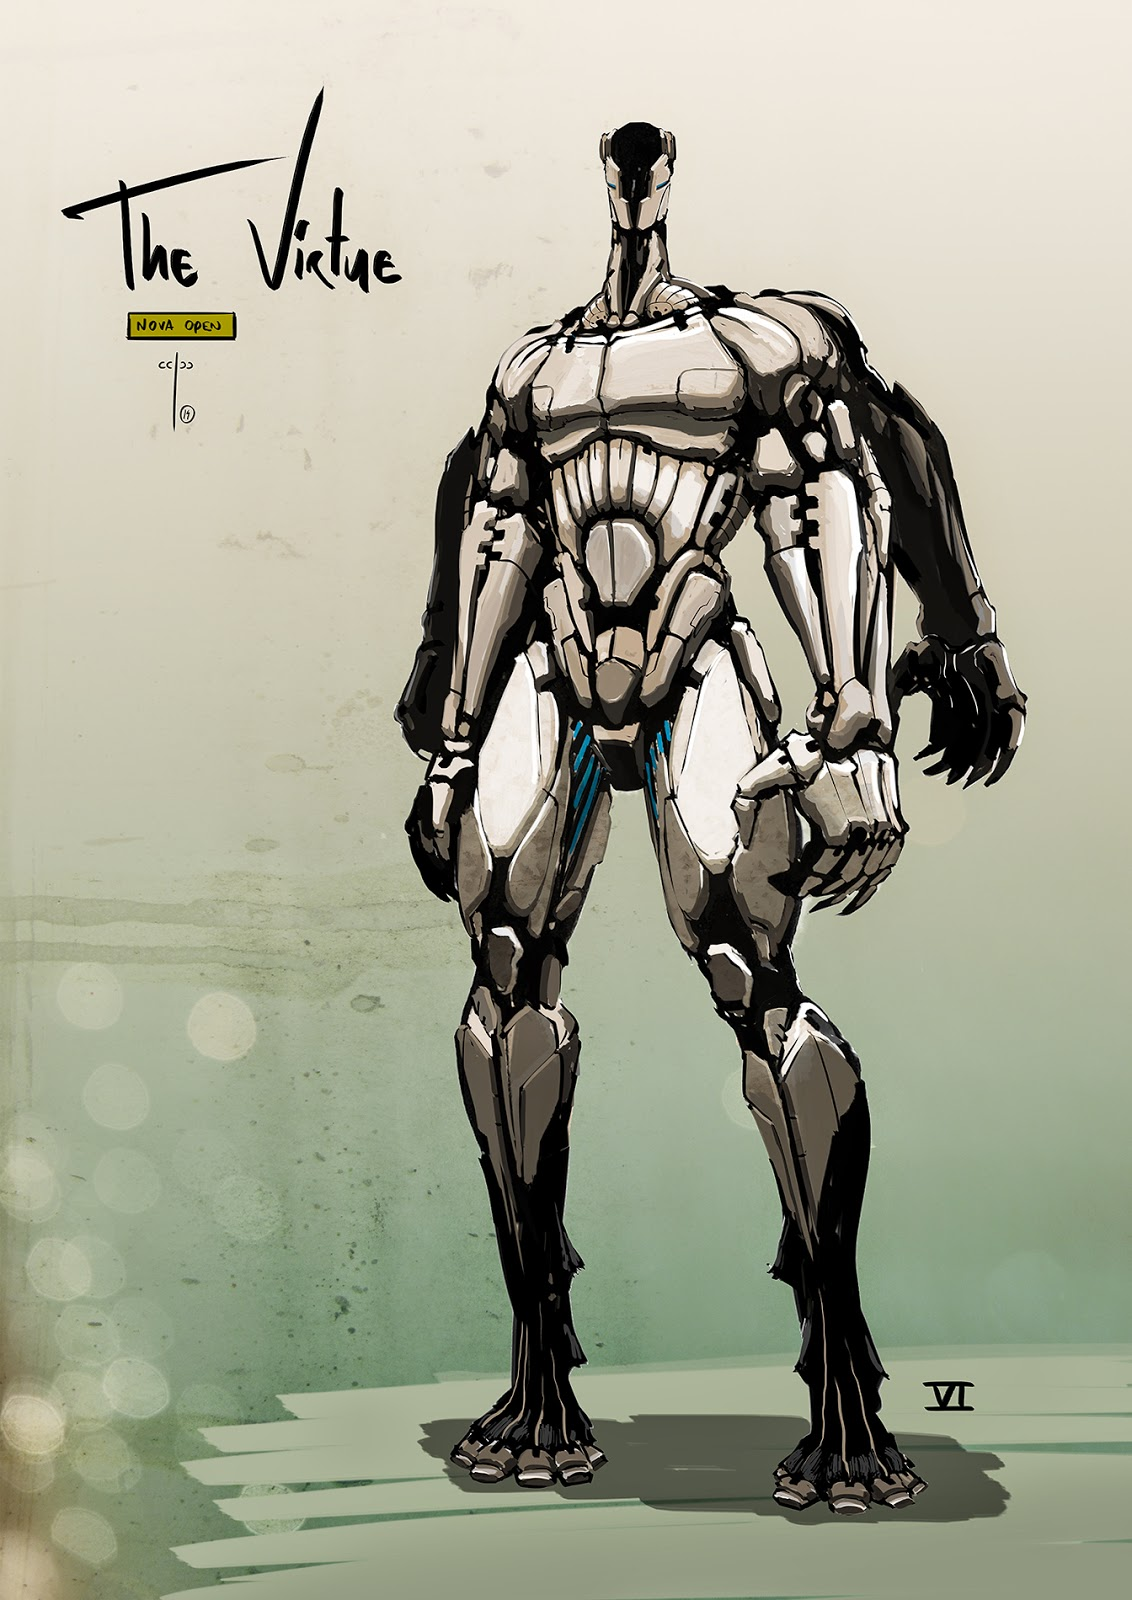
\includegraphics[width=\linewidth]{art/characters/virtue-warrior.jpg}
\end{minipage}

\paragraph{NOVA 2015: Ascension.}  Building on their successes,
humanity's remaining military focused their efforts on the war in
space.  A massive invader space station was discovered and captured,
yielding access to the Bend gates through which they warped time and
space to travel the void.  Meanwhile, ground forces fought to rescue
and protect what remnants of Earth's remaining population they could.
Although a tremendous evacuation was enacted, its scale was tragically
dwarfed by all those necessarily left behind.  Their hand forced by
the ongoing fighting, the survivors waited as long as they could
before closing and destroying the Bend gate inbound to Earth before
launching on their exodus through the outward gate into the stars...

\section{The Virtue}

The alien invaders that beset Earth in~2212 were eventually revealed
as warriors of The Virtue.  For thousands of years The Virtue have
ruled much of the galaxy, encompassing innumerable worlds and species.
Built on fundamental, inarguable virtues and morals, over millenia the
tenets of their society have progressed to become part of their
collective genetic makeup itself.  The Virtue society can do no wrong,
and its citizens need not question if they might do wring in following
its dictates.

As such, none of The Virtue warriors encountered in the fighting over
Earth had ever questioned their task.  For all of known history The
Virtue had stood in judgement over all the fledgeling races of the
galaxy.  As those species reached the threshold of relevance, The
Virtue applied a standard protection and inclusion protocol: Were they
a destructive cancer to be eliminated, or a desirable new element to
be incorporated into The Virtue?  Humanity was simply found wanting,
no further explanation needed.

But those colossal, four-armed warriors encountered on Earth are but
one face of The Virtue, just one of its militaries tasked with
pacifying young races.  The Virtue society is truly vast, and deep
within its governance structures another conclusion had been derived
from the protocols.  From that initial crack, the events at Earth have
slowly emerged as a growing fault line in the very foundations of The
Virtue society.  Never before has The Virtue been turned back from its
objectives, least of all by such an insignificant young race as
Humanity.  For those that have truly considered the implications, the
sheer outrageousness of the defeat calls into question the very
essence of The Virtue.  Eons-old civilizations don't fall often or
easily, but when they do, it comes from doubts such as these.

\section{The Future}

\clearpage
\squelchbackground
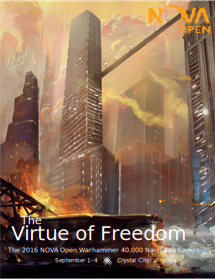
\includepdf[pages={1},fitpaper,offset=0cm 0cm]{art/back/back}
\pagebreak
\restorebackground

%\chapter{Timeline}

\end{document}













There are



humanity in 



gives 

Three paths:

The Path of Daggers

Even the smallest of daggers can cause the gravest of wounds if they
come from behind.

- Attribution lost, The Chronicle of Foundation, sealed historical draft


The Path of Stone

Like a builder who cares only of paint colors, the enclaves too easily
forget the beings, the planets that are the stone foundations of our
society.

- Philosopher-in-exile 


The Path of Blood

War is easy.  Like fighting a v\"o, you cut out the heart and watch
the blood run out.

- Commandant P'Tika





The Virtue
The Coalition of the Free, or The Free as they're more popularly known.

Icons

Virtue: Couple dots, radar-ish circles

Free: Arrows in all directions


Daggers: There's a traitor among the Virtue.  Capture/protect or eliminate

Stone: Control the planets of the sector, by making the population happy or
conquering territory

Blood: Find the rebel base


Final round: Either or both of fighting to take over the Bend station,
or the rebel base

Dagger path pushes toward fighting the bend station
Blood path pushes toward fighting the rebel base
Stone path provides oomph toward either
